% -*- root: ../GeometriaDiferencial.tex -*-
\section{Diferentiable Manifolds}

\begin{problem}[1]
Demuestra que el plano proyectivo es una variedad diferenciable.
\solution
\textcolor{blue}{Este ejercicio está prácticamente resuelto en teoría (\ref{defPlanoProj}) pero lo repetimos aquí con más detalle.}

Recordamos que, por definición, un conjunto $X$ es una variedad diferenciable (\ref{defVariedadDiferenciable}) si cumple:
\begin{enumerate}
\item $X$ es un espacio topológico con topología conexa y Hausdorff.
\item $U_i ⊂ X$ es una familia numerable de abiertos con aplicaciones $\appl{Φ_i}{U_i}{ℝ^n}$, homomorfismos sobre sus imágenes. El par $(U_i, Φ_i)$ es una carta coordenada.
\item Para todo par de de cartas coordenadas $U_i, U_j$ de la estructura diferencial\footnote{Una variedad queda unívocamente definida por un atlas maximal. Un atlas maximal es un atlas que contiene a todos los atlas que son compatibles con él. Dos atlas son compatibles si son equivalentes} y sus correspondientes homomorfismos $Φ_i, Φ_j$, la función $ \inv{Φ_i} ○ Φ_j $ es difeomorfismo en el entorno en el que está definida (en $U_i ∩ U_j$).
\end{enumerate}

Por otro lado tenemos el plano proyectivo definido como:
\[ \projp^2 ≝ \quot{ℝ^3 \setminus \set{0}}{\sim} \]
donde $\sim$ es una relación de equivalencia definida de la siguiente forma: dados $e, e' ∈ ℝ^3$, están relacionados $e \sim e'$ si y sólo si $∃λ ≠ 0$ tal que $λe = e'$.

Primero hay que dotar de una topología a este espacio. Para ello vamos a definir unos conjuntos:

\[U_i = \{(x_1,x_2,x_3) : x_i ≠ 0\}\]

Esta construcción permite decir que $\projp^2(ℝ) = \displaystyle\bigcup_{i=1}^3 U_i$. En cada conjunto se puede construir el homomorfismo $\appl{Φ_i}{U_i}{ℝ^2}$ llevando $[x_0, x_1, x_2]$ a $\left[\frac{x_0}{x_i},\frac{x_1}{x_i},\frac{x_2}{x_i}\right]$. Dado que una de las coordenadas va a ser $1$ siempre, podemos quitarla y entonces será equivalente a $ℝ^2$.

Definimos la topología del plano proyectivo como:

\[ A⊂U_i, A∈\topl \dimplies Φ_i(A) ∈\topl_{ℝ^n}\]

es decir, un subconjunto de $U_i$ es abierto si y sólo si su imagen por $Φ_i$ es un abierto en $ℝ^n$ con la topología habitual. No es de este curso comprobar que esto realmente define una topología ni que esta topología sea la topología con más abiertos tal que la aplicación $\appl{π}{\real^3 \setminus \set{0}}{\projp^2}$ es continua\footnote{$π$ es la combinación apropiada de $Φ_i$ para que sea continua. Es como la proyección en el plano proyectivo utilizado todas las $Φ_i$}.

Esta topología es conexa y Hausdorff, y también compacta.

Al tener una topología conexa y Hausdorff, el plano proyectivo es una variedad topológica.

Tendríamos que comprobar la tercera propiedad de variedad diferenciable. Para ello vemos que el plano proyectivo tratado como variedad tiene tres cartas, dadas por $(U_i,Φ_i)$.

Si tomamos dos cartas $(U_i, Φ_i), \ (U_j, Φ_j)$ vemos que la intersección de los $U$ es:
\[W = U_i \cap U_j= \{(x_1,x_2,x_3): \ x_i \neq 0 \ x_j \neq 0\}\]

Veamos como se comporta la aplicación $ \inv{Φ_i} ○ Φ_j $  sobre $W$:
\[\inv{Φ_i} ○ Φ_j (W)= \inv{Φ_i} \left(\left\{ \left(\frac{x_1}{x_j}, \frac{x_2}{x_j},\frac{x_3}{x_j}\right)\right\}\right) = \left\{ \left(\frac{x_i \cdot x_1}{x_j}, \frac{x_i \cdot x_2}{x_j},\frac{x_i \cdot x_3}{x_j}\right)\right\} \] con $i,j \in \set{1,2,3}$.

Puesto que partimos de la premisa de que $x_i, x_j \neq 0$ tenemos que la función es claramente diferenciable\footnote{cada coordenada es un polinomio de varias variables con un posible denominador no nulo} y puede comprobarse fácilmente que es biyectiva.

La inversa de esta función sería $ Φ_i ○ \inv{Φ_j}$ que se comportaría de la siguiente forma:
\[Φ_i ○ \inv{Φ_j}\left( \{(y_1, y_2, y_3)\}\right) =Φ_i  \left( \{y_1x_j, y_2x_j, y_3x_j\}\right) = \left\{ \left(\frac{y_1x_j}{x_i}, \frac{y_2x_j}{x_i}, \frac{y_3x_j}{x_i} \right)\right\}\]

Esta función sólo estará definida en aquellos puntos en que $x_i\neq$ por lo que resulta ser también diferenciable y vuelve a ser sencilla la comprobación de que la función es biyectiva por lo que queda claro que es un difeomorfismo y por tanto \textbf{el plano proyectivo es una variedad diferencial}.

\end{problem}

\begin{problem}[3] Sea $\appl{γ}{M}{N}$ una aplicación diferenciable. Demuestra que la definición de la diferencial $\appl{\dif γ_p}{\tgs_p M}{\tgs_{γ(p)} N}$ de γ en $p$ no depende de la elección de la curva y que $\dif γ_p$ es una aplicación lineal.

\solution
\textcolor{blue}{Hecho por Pedro. No fiarse al 100\%}

Por definición tenemos
\[dγ_p(v) \in \tgs_{α(p)} N = (γ\circ α)'(0)\]
siendo
\[\appl{α}{(-ε, ε)}{M} \text{ con } α(0)=p, α'(0)=v\]

Sabemos que
\[(γ\circ α)'(0) = α'(0)(γ'(α(0)) = v \cdot γ'(p)\]

sin importar la curva $α$ tomada siempre y cuando cumpla las condiciones pedidas.

Ahora es sencillo ver que es lineal pues tenemos que es una aplicación que, dado un vector $v$ nos lleva a ese mismo vector multiplicado por un valor constante por lo que es lineal de manera trivial.
\end{problem}

\begin{problem}[4]
Let $\appl{γ}{M}{N}$ be an inmersion and let $p$ be a point in $M$. Show that there exists a neighborhood $V \subset M$ of $p$ such that the restriction $γ|_V$ is an embedding (This means that every inmersion is locally an embedding).

\solution
\textcolor{blue}{Hecho por Pedro. No fiarse al 100\%}

Para empezar recordemos lo que era una \textbf{inmersión}: Sean $M$ y $N$ variedades diferenciables. Se dice que una función diferenciable $\appl{F}{M}{N}$ es una \textbf{inmersión} en $p$ si la diferencial $\appl{F_{*p}}{\tgs_pM}{\tgs_{F(p)}N}$ entre los espacios tangentes es inyectiva. Si $F$ es una inmersión para todo punto $p\in M$ decimos que es una \textbf{inmersión}.

Recordemos también lo que era un \textbf{embedding}: Si una \textbf{inmersión} es un homeomorfismo sobre su imagen, con la topología inducida en esta por $N$, decimos que es un \textbf{embedding}

Puesto que toda función diferenciable es continua podemos tomar un entorno de $γ(p)$ y calcular su preimagen, que será un entorno de $p$. La restricción de γ a este entorno será inyectiva, por ser inyectiva γ en general y será sobreyectiva por construcción por lo que será biyectiva. Así podemos garantizar que tendrá inversa diferenciable y por tanto se trata de un homeomorfismo sobre su imagen lo que implica que γ es un \textbf{embedding}
\end{problem}
\newpage
\begin{problem}[6]
Consider the cylinder $C=\{(x,y,z) \in \real^3 \tq x^2+y^2=1\}$ and indentify the point $(x,y,z)$ with $(-x,-y,-z)$. Show that the quotient space of $C$ by this equivalence relation can be given a differentiable structure. (infinite Möbius band)
\solution

\textcolor{blue}{Hecho por Pedro. No fiarse al 100\%}

Primero mostramos un ejemplo encontrado por internet que resuelve un problema muy similar a este.

\begin{center}
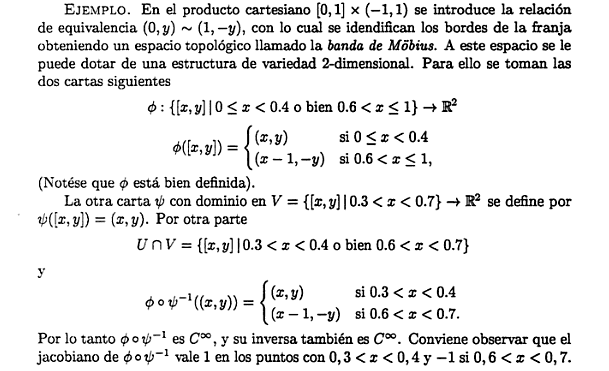
\includegraphics[keepaspectratio=true,width=\linewidth]{img/ejemplo_6.png}
\end{center}

Para dotar a un conjunto de estructura diferencial basta con encontrar un atlas para el cual se cumpla la definición de estructura diferencial sobre el conjunto dado.

Tomamos 8 cartas de la siguiente forma:
\begin{enumerate}
\item
\[\appl{\phi_1}{\{(x,y,z) \tq x\in [0,1), y \in [0,1), z \geq 0\}}{\real^3}\]
siendo $\phi_1=Id$
\item
\[\appl{\phi_2}{\{(x,y,z) \tq x\in (-1,0], y \in [0,1), z \geq 0\}}{\real^3}\]
siendo $\phi_2([x,y,z])=(-x,y,z)$
\item
\[\appl{\phi_3}{\{(x,y,z) \tq x\in [0,1), y \in (-1,0], z \geq 0\}}{\real^3}\]
siendo $\phi_3([x,y,z])=(x,-y,z)$
\item
\[\appl{\phi_4}{\{(x,y,z) \tq x\in [0,1), y \in [0,1), z \leq 0\}}{\real^3}\]
siendo $\phi_4([x,y,z])=(x,y,-z)$
\item
\[\appl{\phi_5}{\{(x,y,z) \tq x\in (-1,0], y \in (-1,0], z \geq 0\}}{\real^3}\]
siendo $\phi_5([x,y,z])=(-x,-y,z)$
\item
\[\appl{\phi_6}{\{(x,y,z) \tq x\in (-1,0], y \in [0,1), z \leq 0\}}{\real^3}\]
siendo $\phi_6([x,y,z])=(-x,y,-z)$
\item
\[\appl{\phi_7}{\{(x,y,z) \tq x\in [0,1), y \in (-1,0], z \leq 0\}}{\real^3}\]
siendo $\phi_7([x,y,z])=(x,-y,-z)$
\item
\[\appl{\phi_8}{\{(x,y,z) \tq x\in (-1,0], y \in (-1,0], z \leq 0\}}{\real^3}\]
siendo $\phi_8([x,y,z])=(-x,-y,-z)$

\end{enumerate}

La combinación de una de estas funciones con la inversa de otra no implicará más que cambios de signo sobre las variables de tal forma que
\[\phi_i\circ \inv{\phi_j}(x,y,z)=(\pm x, \pm y, \pm z)\]

Buscamos que estas combinaciones sean difeomorfismos en el entorno en el que están definidas (la intersección de sus dominios) (\ref{defVariedadDiferenciable}) y queda claro que estas aplicaciones son $C^{\infty}$ y sus inversas, que son de la misma forma, también. Conviene observar que el jacobiano vale siempre $\pm 1$.

Por ejemplo, $Φ_7\circ Φ_8^{-1} (-x,-y,-z) = Φ_7([x,y,z]) = (x,-y,-z)$ en $U_7 ∩ U_8 = \{(x,y,z) \tq x=0, y∈(-1,0], z≤0\}$.
\end{problem}

\section{fasc-4-ejemplos}

\subsection{Variedades}
\begin{problem}[2]
Estudiar, siguiendo el modelo de $S^2$ la estructura de variedad diferenciable, con dos cartas, en $S^n$

\solution
\textcolor{blue}{Hecho por Pedro. No fiarse al 100\%}

Comenzamos considerando una esfera de radio 1 en $\real^n$ que tendrá la ecuación:
\[\sum_{i=1}^n x_i^2=1\]
y describiendo explícitamente el atlas de dos cartas dado por la proyección estereográfica.

Siguiendo el ejemplo de la hoja, consideramos la proyección tomando el polo norte $(1,0...0)$ y el plano $x_1=-1$. Posteriormente construiremos la segunda carta tomando el polo sur $(-1,0...0)$ y el plano $x_1=1$. Vamos a ello.

\textbf{Primera carta}

\begin{itemize}
\item Supongamos un punto $p$ cualquiera del plano $x_1=-1$:
\[p=(-1,x_2,...x_n)\]

Si construimos la recta que lo une con el polo norte y la intersecamos con la esfera $S^n$ obtenemos el punto intersección $q$.
\[q = \left(1-2t, x_2\cdot t,...,x_n\cdot t\right)\]
Si el punto es la intersección con la esfera, su módulo deberá ser 1. Utilizamos este dato para calcular $t$.

\[1+4t^2-4t+t^2\left(\sum_{i=2}^nx_i^2\right)=1 \implies 4t^2-4t+t^2\left(\sum_{i=2}^nx_i^2\right) = 0 \implies t=\frac{4}{\sum_{i=2}^nx_i^2+4}\]

Por tanto el punto de intersección es:
\[q=\left(1-\frac{8}{\sum_{i=2}^nx_i^2+4}, \frac{4x_2}{\sum_{i=2}^nx_i^2+4},...,\frac{4x_n}{\sum_{i=2}^nx_i^2+4} \right)\]

\item Al revés. Empezamos ahora con un punto
\[x\in S^n\tq x=(α_1...α_n) \text{ con } \sum_{i=1}^n α_i^2 = 1\]

Construimos ahora el vector que une este punto con el polo norte y lo intersecamos con el plano $x_1=-1$

La recta unión con el polo norte queda de la forma:
\[\left(1+t(α_1+1),α_2t,...,α_nt \right)\]
y forzamos la intersección de esta recta con el plano para conocer el punto
\[1+t(α_1+1)=-1 \implies t = \frac{-2}{α_1+1}\]
con lo que el punto sería:
\[\left( -1, \frac{-2α_2}{α_1-1}, ..., \frac{-2α_n}{α_1-1}\right)=\left( -1, \frac{2α_2}{1-α_1}, ..., \frac{2α_n}{1-α_1}\right)\footnote{En el ejmplo de la hoja creo que escriben $α_1$ en función de las otras coordenadas, pero no veo necesaria esta complicación}\]
\end{itemize}

\textbf{Segunda carta}
\begin{itemize}
\item Supongamos un punto $p$ cualquiera del plano $x_1=1$:
\[p=(1,x_2,...x_n)\]

Si construimos la recta que lo une con el polo sur y la intersecamos con la esfera $S^n$ obtenemos el punto intersección $q$.
\[q = \left(-1+2t, x_2\cdot t,...,x_n\cdot t\right)\]
Si el punto es la intersección con la esfera, su módulo deberá ser 1. Utilizamos este dato para calcular $t$.

\[1+4t^2-4t+t^2\left(\sum_{i=2}^nx_i^2\right)=1 \implies 4t^2-4t+t^2\left(\sum_{i=2}^nx_i^2\right) = 0 \implies t=\frac{4}{\sum_{i=2}^nx_i^2+4}\]

Por tanto el punto de intersección es:
\[q=\left(-1+\frac{8}{\sum_{i=2}^nx_i^2+4}, \frac{4x_2}{\sum_{i=2}^nx_i^2+4},...,\frac{4x_n}{\sum_{i=2}^nx_i^2+4} \right)\]

\item Al revés. Empezamos ahora con un punto
\[x\in S^n\tq x=(α_1...α_n) \text{ con } \sum_{i=1}^n α_i^2 = 1\]

Construimos ahora el vector que une este punto con el polo sur y lo intersecamos con el plano $x_1=1$

La recta unión con el polo sur queda de la forma:
\[\left(-1+t(α_1+1),α_2t,...,α_nt \right)\]
y forzamos la intersección de esta recta con el plano para conocer el punto
\[-1+t(α_1+1)=1 \implies t = \frac{2}{α_1+1}\]
con lo que el punto sería:
\[\left( 1, \frac{-2α_2}{α_1+1}, ..., \frac{-2α_n}{α_1+1}\right))\]
\end{itemize}

Estudiamos ahora un punto cualquiera del plano $(-1,...x_n)$. Si lo mandamos en la esfera por la primera proyección que hemos calculado, llegamos al punto
\[\left(1-\frac{8}{\sum_{i=2}^nx_i^2+4}, \frac{4x_2}{\sum_{i=2}^nx_i^2+4},...,\frac{4x_n}{\sum_{i=2}^nx_i^2+4} \right)\]

Ahora calculamos la imagen directa de este punto por la segunda proyección estereográfica, con lo que llegamos a:
\[\left( 1, \frac{-2\frac{4x_2}{\sum_{i=2}^nx_i^2+4}}{2-\frac{8}{\sum_{i=2}^nx_i^2+4}}, ..., \frac{-2\frac{4x_n}{\sum_{i=2}^nx_i^2+4}}{2-\frac{8}{\sum_{i=2}^nx_i^2+4}}\right)=\left( 1, \frac{-4x_2}{\sum_{i=2}^nx_i^2},...,\frac{-4x_n}{\sum_{i=2}^nx_i^2}\right)\]

y podemos ver que se trata de un difeomorfismo sobre su imagen

\textcolor{blue}{En algún punto he metido la gamba con los signos porque debería salirme todo positivo. Pero ya he currado mucho con este ejercicio. Una paja y a seguir.}

\end{problem}



\begin{problem}[3]
Parametrizamos los puntos del hemisferio norte de la esfera $x_2 > 0$,
excluyendo el ecuador ($x_2 = 0$), en la forma $(θ, τ, + \sqrt{1 − θ^2 − τ^2})$ con
$θ^2 + τ^2 < 1$. Esto convierte al hemisferio norte en una carta coordenada, y podemos cubrir la esfera con seis cartas de este tipo tomando
como ecuador cada una de las intersecciones de la esfera con los planos
coordenados. COMPROBAR que, efectivamente, se trata de un atlas.

DEMOSTRAR que los dos atlas son equivalentes, viendo que los cambios
de carta de una carta de uno de ellos a una carta del otro inducen difeomorfismos.

\solution
\end{problem}

\begin{problem}[4]
Demostrar que no existe ninguna variedad diferenciable compacta que se pueda recubrir con una única carta coordenada
\solution

\textcolor{blue}{Hecho por Pedro. No fiarse al 100\%}

Si una variedad se puede recubrir por una única carta será homeomorfa a un abierto de $\real^n$ y, consecuentemente, nunca podrá ser compacta.

Esta respuestá está basada en la proposición 1.28 del documento: \href{http://ocw.um.es/ciencias/geometria-y-topologia/material-de-clase-1/01-variedadesdiferenciablessubvariedades-v100901.pdf}{Variedades Diferenciales y Subvariedades.pdf}
\end{problem}

\begin{problem}[5]
Demostrar que toda variedad 1-dimensional compacta y conexa es difeomorfa a la circunferencia $S^2$
\solution

\textcolor{blue}{Hecho por Pedro. No fiarse al 100\%}

Para empezar es obvio que en caso de haber un difeomorfismo entre una variedad y la circunferencia, la variedad ha de ser compacta y conexa, pues así lo es la circunferencia.

Para resolver este ejercicio me baso en la proposición VI.1.6 de \href{https://books.google.es/books?id=CAOjRFAMJFUC&pg=PA131&lpg=PA131&dq=variedad+1-dimensional&source=bl&ots=MLkMP7HMyo&sig=aLLSSaYknqPZhPsn-5jJM2MwPAc&hl=es&sa=X&ei=DeMeVZSOEczZPdLkgfgJ&ved=0CCcQ6AEwAQ#v=onepage&q&f=false}{documento.pdf}. Básicamente la copio como un bellaco pero ahí dejo el link para el que quiera profundizar.

\textcolor{blue}{Justo en la versión que se puede consultar gratis en Google han quitado las dos páginas clave en que salía esto. El lunes pillo el libro en ciencias y lo completo}

\end{problem}

\begin{problem}[6]
Demostrar, como consecuencia del teorema de invarianza del dominio, que si $n \neq m$, no pueden ser homeomorfos $\real^n$ y $\real^m$. Tampoco es posible que sean homeomorfos un abierto de $\real^n$ con uno de $\real^m$
\solution

\textcolor{blue}{Hecho por Pedro. No fiarse al 100\%}

En el fascículo 2 que podemos encontrar en moodle aparece la demostración de este hecho, que repetimos a continuación.

Supongamos abiertos $U \subset \real^n$ y $V\subset \real^m$ y la función $\appl{F}{U}{V}$ un difeomorfismo, es decir, una aplicación biyectiva, infinitamente diferenciable y con inversa infinitamente diferenciable.

\begin{enumerate}
\item Consideramos la función $G$ que es la función inversa de $F$, de forma que $G \circ F = 1_U$ y $F \circ G = 1_V$ siendo $1_X$ la identidad dentro del conjunto $X$.

\item Aplicando la regla de la cadena obtenemos:
\[G_{*,F(p)}\circ F_{*,p} = (1_U)_{*,p} \text{ y }  F_{*,p} \circ G_{*,F(p)} = (1_V)_{*,F(p)}\]

\item Pero, puesto que la matriz de la diferencial es la matriz jacobiana sabemos que
\[(1_U)_{*,p} = 1_{\tgs_p} \text{ y } (1_V)_{*,F(p)} = 1_{\tgs_{F(p)}}\]

\item Puesto que las aplicaciones $F_{*,p}$ y $G_{*,F(p)}$ son inversas la una de la otra los espacios $\tgs_p$ y $ 1_{\tgs_{F(p)}}$ son necesariamente isomorfos y por tanto $n$ y $m$ son iguales
\end{enumerate}

De hecho es imposible un \textbf{homomorfismo} entre abiertos de $\real^n$ y $\real^m$ pero esto se trata de un resultado topológico cuya demostración no entraría en el temario de este curso.

No obstante podemos encontrar esta última demostración en el siguiente \href{http://www.cmat.edu.uy/~rpotrie/documentos/pdfs/invarianciadimension.pdf}{documentopdf}
\end{problem}

\begin{problem}[7]
Demostrar que, si $\appl{f}{M}{N}$ es una función continua y localmente inyectiva de variedades topologícas de dimensión $n$, entonces la imagen de todo abierto $U \subset M$ es un abierto de $N$. En particular, $f(M)\subset N$ debe ser un abierto, que puede ser toda la variedad $N$
\solution

\textcolor{blue}{Hecho por Pedro. No fiarse al 100\%}

Esto es un resultado de Topología que no voy a rehacer ya que no le veo mucha relación con lo que estamos estudiando en esta asignatura.

Por comentar algo relacionado con lo que estamos viendo, he viso en Wikipedia, y cito textualmente: ``El teorema de la invariancia del dominio establece que una función continua y localmente inyectiva entre dos variedades topológicas n-dimensionales debe ser abierta.''
\end{problem}

\begin{problem}[8]
Sea $S$ el conjunto de sucesiones $\appl{σ}{\nat}{\real}$ de números reales.

Definimos una topología en $S$ exigiendo que todas las funciones naturales de proyección
\[\appl{μ_{i_1,i_2,...,i_n}}{S}{\real^n}\]
sean continuas.\footnote{Estas funciones básicamente llevan la sucesión a un vector de $\real^n$ formado por $n$ elementos de la sucesión.}

Definimos una función $\appl{F}{S}{S}$ mediante
\[F(x_0,x_1,...,x_n,...)=(x_1,x_2,...,x_n,...)\]
Demostrar que la función $F$ es continua e inyectia, pero su imagen no es un abierto de $S$

\solution


\end{problem}

\begin{problem}[9]
Sea $U$ una bola unidad abierta en $\real^n$. Comprobar que la aplicación
\[f(\vx)=\frac{\vx}{\sqrt{1-\norm{\vx}^2}}\]
es un difeomorfismo de $U$ en todo $\real^n$
\solution

\yoP

Para comprobar que $f$ es un difeomorfismo debemos ver que es diferenciable, biyectiva y con inversa diferenciable. Vamos a ello.

La función, descompuesta en coordenadas, queda de la forma:
\[f(\vx)=\left(\frac{x_1}{\sqrt{1-\norm{\vx}}}, \frac{x_2}{\sqrt{1-\norm{\vx}}}, ..., \frac{x_n}{\sqrt{1-\norm{\vx}}}\right)\]

Vamos a derivarla:
\[\frac{\partial f}{\partial x_i}=\left(\frac{x_1x_i}{(\sqrt{1-\norm{\vx}})^3},\frac{x_2x_i}{(\sqrt{1-\norm{\vx}})^3},..\frac{1}{\sqrt{1-\norm{\vx}}}+\frac{x_i^2}{(\sqrt{1-\norm{\vx}})^3}.,\frac{x_nx_i}{(\sqrt{1-\norm{\vx}})^3}\right)\]

Podemos observar que la derivada existe (y por tanto la función es diferenciable) en todo punto con norma distinta de 1. Puesto que nos estamos restringiendo a $U$ que es la bola unidad \textbf{abierta} no hay problema con esto.

Podemos ver de manera sencilla que la función es inyectvia pues la derivada nunca se anula y podemos ver que es sobreyectiva por contrucción. Para cualquier punto de $\real^n$ que tomemos podemos escribirlo como $f(\vx)$\footnote{Esto queda claro al calcular la función inversa, cosa que haremos a continuación}.

Por último nos queda estudiar la inversa.

\[f(\vx)=\vy \implies (y_1,....y_n)=\left(\frac{x_1}{\sqrt{1-\norm{\vx}}}, \frac{x_2}{\sqrt{1-\norm{\vx}}}, ..., \frac{x_n}{\sqrt{1-\norm{\vx}}}\right)\]

A ojo de buen cubero podemos ver que la función inversa sería
\[f^{-1}(\vy)=\frac{\vy}{\sqrt{1+\norm{\vy}}}\]
cosa que podemos comprobar fácilmente.

Resulta también trivial la observación de que esta función inversa también es diferenciable, por lo que queda claro que $f$ es un difeomorfismo.

\end{problem}


\subsection{Campos}
\begin{problem}[1]
(\textbf{Grupos uniparamétricos de automorfismos}) En cada uno de los siguientes ejemplos se da una familia uniparamétrica de automorfismos de $\real^n$ y se pide que se compruebe que es un grupo y determine el campo asociado (\textbf{generador infinitesimal del grupo}). En todos los casos el grupo es un grupo de transformaciones lineales y el campo es un campo lineal (coeficientes de grado a lo más uno)

\ppart Grupo de traslaciones
\[τ_1(x_1,...,x_n)=(x_1+t,x_2,...,x_n)\]

\ppart Grupo de homotecias
\[τ_t(x_1,...,x_n)=(e^tx_1, e^tx_2,...,e^tx_n\]

\ppart Sea $A$ una matriz $n\times n$. Definimo un grupo uniparamétrico de automorfismos, asociado a la matriz $A$, mediante
\[τ_t(X)=e^{tA}X\]
¿Es el primer ejemplo un caso particular de este?

\ppart
Supongamos ahora $n=2$, y sea
\[ \left( \begin{array}{cc}

\cos(t) & -\sin(t) \\
\sin(t) & \cos(t)

\end{array} \right)\]
la matriz de una rotación de ángulo variable $t$ en el plano. Definimos un grupo uniparamétrico de automorfismos
\[τ_t(x_1,x_2)=A(t)\cdot {x_1 \choose x_2}\]

¿Es este ejemplo un caso particular del c)?

\solution
\yoP

Para demostrar que cada uno de estos conjuntos es un grupo debemos identificar la operación que define el grupo, demostrar que es asociativa y encontrar el elemento neutro o identidad y el inverso.

\spart
La operación suma se define de la siguiente forma:
\[(τ_a+τ_b)(x_1,...,x_n)=(x_1+a+b,x_2,...,x_n)\]

Es evidente que la operación es asociativa, el elemento neutro es $τ_0$ y el inverso de $τ_t$ es $τ_{-t}$

Queda claro que es un grupo.

Vamos a encontrar el campo asociado. La teoría de lo que vamos a hacer a continuación viene en las páginas 73-74 de \href{http://matematicas.unex.es/~ricarfr/EcDiferenciales/LibroEDLat.pdf}{documento.pdf}

Básicamente nos da un teorema y su demostración. El teorema dice:

Sea $X$ un grupo uniparamétrico local de clase $k$. Para cada $f\in C^{\infty}(U)$ y $p \in U$ definimos
\[(Df)(p)=\lim_{t \to 0}\frac{f[X(t,p)]-f(p)}{t}\]
entonces $D \in D_k(U)$ y lo llamaremos generador infinitesimal de X.

El ejemplo concreto que vamos a hacer (o uno muy similar) así como los siguientes vienen resuletos al final de la página 16 de \href{http://matematicas.unex.es/~ricarfr/EcDiferenciales/LibroEDLat.pdf}{documento.pdf}

Así para este ejemplo tendríamos la aplicación flujo $\appl{\phi}{\real^{n+1}}{\real^n}$ siendo $\phi(x_1,...,x_n,t)=(x_1+t,x_2,...,x_n)$.

\[X = \left(\frac{\partial \phi}{\partial t}\right)_{t=0} \frac{\partial}{\partial x_i}=\frac{\partial}{\partial x}\]


\textbf{Del último documento mencionado cabe destacar:}

\begin{defn}[Generador\IS infinitesimal]
Sea $\{σ_t\}$ un grupo monoparamétrico de transformaciones de U. Llamamos \textbf{generador infinitesimal} de $\{σ_t\}$ al campo vectorial que asigna al punto $p$, el vector tangente a la curva $(-ε,ε)\to U$, $t \to σ_t(p)$

Consideremos $\appl{\phi}{\real \times U}{U}$ la aplicación flujo del grupo $\phi(t,p)=σ_t(p)$. entonces el generador infinitesimal puede considerarse
\[X = \sum_{i=1}^n \left( \frac{\partial \phi_i}{\partial t}\right)_{t=0}\frac{\partial}{\partial x_i}\]
\end{defn}

\end{problem}

\begin{problem}[2]
Sea $D$ el campo en $\real^2$ definido como
\[D=x \frac{\partial}{\partial x}+y \frac{\partial}{\partial y }\]

El campo está definido en todo el plano pero

\ppart Una integral primera definida en todo el plano es necesariamente constante

\ppart Para cada punto, diferente al origen hay un entorno en el que hay una integral primera. Determinar todas esas integrales primeras no globales y los abiertos máximos en que están definidas.
\solution


\yoP

\spart
Vamos a tratar de resolver y buscar la integral primera: funciones $H$ tales que $D(H) = 0$. Para ello, resolvemos el par de ecuaciones
\begin{align}
\frac{\partial H}{\partial x} &= \frac{1}{x} \implies H(x,y)=\log(x)+f(y)\\
\frac{\partial H}{\partial y} &= \frac{1}{y} \implies H(x,y)=\log(y)+g(x)
\end{align}

De donde concluimos que $H(x,y)=\log(x)+\log(y)$. El problema de esta integral primera es que no está definida en todo el plano.

Tenemos que buscar otra forma de encontrar integrales primeras definidas en todo el plano. Para ello resolvemos el sistema
\begin{align}
\frac{\partial H}{\partial x} &= -y \implies H(x,y)=-xy+f(y)\\
\frac{\partial H}{\partial y} &= x \implies H(x,y)=yx+g(x)
\end{align}

No hay elección posible de $C_1$ y $C_2$ que resuelva ese sistema. Sin embargo, el campo es no nulo en todo punto salvo en $(0,0)$, y tienen que existir integrales primeras en entornos de esos puntos. Así, sólo nos queda una opción, que $\dpa{H}{x} = \dpa{H}{y} = 0$, luego $H(x,y)$ tiene que ser constante.

Otro punto de vista es el siguiente: si resolvemos el sistema de EDOs asociado \begin{align*}
x'(t) &= x(t) \\
y'(t) &= y(t)
\end{align*} nos queda que las curvas solución son de la forma $γ(t) = (c_1e^t, c_2e^t)$. Cuando $t = 0$, $γ(0) = (c_1, c_2)$ luego está claro que las constantes son las coordenadas del punto inicial de la curva $(x_0, y_0) = (c_1, c_2)$.

Haciendo el corte de γ con el plano $x = 1$, tenemos \[ 1 = x_0e^t \implies t = - \log x_0 \], y sustituyendo en la ecuación de la segunda coordenada queda $y = \frac{y_0}{x_0}$, que efectivamente son curvas constantes.

\spart Retomamos el primer cálculo de integral primera que hicimos: $H(x,y)=\log(x)+\log(y)$

Estas integrales primeras están definidas en todo punto salvo en los ejes de coordenadas.

\end{problem}

\begin{problem}[3]
Estudiar el campo en el plano definido como
\[D=(y+x(1-x^2-y^2))\frac{\partial}{\partial x} + (-x+y(1-x^2-y^2))\frac{\partial}{\partial y}\]
usando, si te parece conveniente, un cambio a coordenadas polares.
\solution
\yoP

Vamos a ver las curvas solución o curvas integrales del campo. Básicamente esto consiste en buscar una función tal que en todo punto su vector tangente sea el dado por D. Es decir, que su derivada coincida con el campo.

Buscamos $\appl{α}{I}{\real^2}$ siendo $α(t)=(x(t),y(t))$, tal que
\begin{align}
\frac{dx}{dt} &= y+x(1-x^2-y^2) \\
\frac{dy}{dt} &= -x+y(1-x^2-y^2)
\end{align}

Dado que esto parece un tanto inmanejable vamos a atender al consejo dado y pasamos todo a coordenadas polares. Así el campo quedaría:
\[D=(r(\sin(\theta)+\cos(\theta)(1-r^2)))\left(\cos(\theta)\frac{\partial}{\partial r} - r\sin(\theta)\frac{\partial}{\partial \theta} \right)+\]
\[+(r(-\cos(\theta)+\sin(\theta)(1-r^2)))\left(\sin(\theta)\frac{\partial}{\partial r} + r\cos(\theta)\frac{\partial}{\partial \theta} \right)\]
operando un poco podemos dejarlo más bonito como:
\[D= r(1-r^2)\frac{\partial}{\partial r}+r^2\frac{\partial}{\partial \theta}\]

En estas condiciones podemos considerar $α(t)=(r(t),\theta(t))$ y al buscar la curva integral nos quedaría el sistema de ecuaciones:
\begin{align}
\frac{dr}{dt} &= r(1-r^2) \implies dt = \frac{dr}{r-r^3} \implies t=\log(r)-\frac{1}{2}\log(1-r^2) \\
\frac{d\theta}{dt} &= r^2 \implies d\theta=\frac{r^2dr}{r-r^2} \implies \theta = -\frac{1}{2}\log(1-r^2)
\end{align}

Si despejamos $t$ de la primera ecuación obtenemos:
\[r= \frac{-1 \pm \sqrt{1+e^t}}{e^t}\]
pero vemos que si tomamos la opción con el signo menos habrá valores de $t$ para los que la $r$ sea negativa lo que nos daría problemas en el $\log(r)$. Por tanto nos queda
\[α(t)=\left(\frac{-1 + \sqrt{1+e^t}}{e^t}, -\frac{1}{2}\log\left(\frac{2-2\sqrt{1+e^t}}{e^{2t}} \right)\right)\]

\textcolor{red}{TRIIIIIIIIIIIIIIIIPLEEEEEEEEEE}
\end{problem}

\begin{problem}[5]
Para cada uno de los campos $D_i$, definido en un abierto $U_i$ encontrar un sistema de coordenadas en el que el campo se endereza

\ppart
\[D_1 = x \frac{\partial}{\partial x}+2y\frac{\partial}{\partial y} \text{ siendo } U_i=\{(x,y) \tq x > 0\}\]

\ppart
\[D_2 = \frac{\partial}{\partial x}+\sin(x)\frac{\partial}{\partial y} \text{ siendo } U_2 = \real^2\]

\ppart
\[D_3 = x\frac{\partial}{\partial x}+(1-x^2)\frac{\partial}{\partial y} \text{ siendo } U_3 = \{(x,y) \tq -1 < x < 1\}\]

\solution

\spart
Para enderezar el campo calculamos su integral primera:
\[0 = D(H) = x\frac{\partial H}{\partial x}+2y\frac{\partial H}{\partial y}\]
Para resolver esta ecuación debemos resolver el sistema:
\begin{align*}
\frac{\partial H}{\partial x} &= -2y\\
\frac{\partial H}{\partial y} &= x
\end{align*}

de donde obtenemos nada porque no sale. Cuando esto no conduce a nada directamente, el remedio es calcular las curvas solución. Resolvemos
\begin{align*}
\od{x}{t} &= x \\
\od{y}{t} &= 2y
\end{align*} y nos da que
\begin{align*}
x(t) &= e^t x(0) \\
y(t) &= e^{2t} y(0)
\end{align*}

Ahora tenemos que cortar estas curvas solución con un plano. No puede ser el plano $x = 0$ porque no pasan por $x = 0$. Cortamos por un plano $y_0$ que no sé qué es, parece que es el punto donde estamos enderezando el campo. Resolvemos
\[ e^{2t} y(0) = y_0 \implies t = \frac{\log y_0 - \log y(0)}{2} \], que sustituyendo en $x(t)$ nos da \[ x = e^{\frac{\log y_0 - \log y(0)}{2}} x(0) = x \sqrt{\frac{y_0}{y(0)}} \] y entonces la función $H$ que buscamos es \[ H(x,y) =  x \sqrt{\frac{y_0}{y}} \]

Para enderezar el campo, hay que aplicar una fórmula de la que el profesor no se acuerda. A veces se ve pero en otros casos hay que hacer una integral de una función de $n$ variables integrando con respecto a una de ellas y en general es horroroso y no lo vamos a ver.

\spart

Para enderezar el campo calculamos su integral primera
\[0 = D(H) = \frac{\partial H}{\partial x}+\sin(x)\frac{\partial H}{\partial y}\]
Para resolver esta ecuación debemos resolver el sistema:
\begin{align}
\frac{\partial H}{\partial x} &= -\sin(x)\\
\frac{\partial H}{\partial y} &= 1
\end{align}

de donde obtenemos $H(x,y)=\cos(x)+y$

Ahora debemos buscar una función $G$ tal que $D(G)=1$ para ello basta con tomar $G(x,y)=x$

¿Determinan las funciones $H$ y $G$ un sistema de coordenadas locales? Para ello debemos estudiar el rango de su matriz jacobiana:
\[\left( \begin{array}{cc}
-\sin(x) & 1  \\
1 & 0  \end{array} \right)\]

y vemos que el determinante es siempre 1 por lo que tenemos un sistema de coordenadas locales en el entorno de cualquier punto del plano. Si conseguimos probar que el cambio de coordenadas es biyectivo, tendremos un sistema de coordenadas definido en todo el plano $\real^2$.

Tenemos pues el cambio de coordenadas:
\begin{align}
x_1 &= \cos(x)+y\\
y_1 &= x
\end{align}

que es claramente invertible siendo:
\begin{align}
x = y_1\\
y = x_1 - \cos(y_1)
\end{align}

Entonces, el campo $D$ se endereza en un sistema de coordenadas definido en todo el plano.

\spart
\yoP

Buscamos nuevamente una función $H$ que sea integral primera del campo. En este caso no es posible calcularla directamente, de modo que tendremos que hacer algo parecido a lo que hacíamos en el apartado \textbf{a)}.

Calculamos directamente la curva solución del campo:
\begin{align}
\dot{x}&=x \implies x(t)=e^tx(0)\\
\dot{y}&=(1-x^2) \implies y(t)=\int 1-e^{2t}x(0)^2 dt \implies y(t)=t-\frac{e^{2t}x(0)^2}{2}+y(0)+\frac{x(0)^2}{2}
\end{align}

Tomamos un punto en el que el campo no se anule como puede ser el punto $(1,0)$. Ahora debemos tomar una hipersuperficie que no contenga al vector $D_p$, que será el plano $x=1$. Veamos en qué punto la curva solución corta a esta hipersuperficie:

\[e^t x(0)= 1 \implies t = \log\left(\frac{1}{x(0)}\right)\]
lo que nos da un valor de la segunda coordenada del punto:
\[y(t)=\log\left(\frac{1}{x(0)}\right)-\frac{1}{2}+y(0)+\frac{x(0)^2}{2}\]

Concluimos que la integral primera del campo sería:
\[H(x,y)=\log\left(\frac{1}{x}\right)-\frac{1}{2}+y+\frac{x^2}{2}\]

Para cercionarnos de que todo está bien podemos comprobar de forma sencilla que $D(H)=0$.

Para terminar de enderezar el campo deberíamos encontrar una función $G$ tal que $D(G)=1$. Para ello basta con tomar $G(x,y)=\log(x)$. Así, nos queda que el cambio de variables que permite enderezar el campo es:
\begin{align}
x_1 = \log\left(\frac{1}{x}\right)-\frac{1}{2}+y+\frac{x^2}{2}
y_1 = \log(x)
\end{align}

Para comprobar en qué puntos este cambio de variables es válido estudiamos el rango de su matriz Jacobiana:

\[\left( \begin{array}{cc}
x-\frac{1}{x} & \frac{1}{x}  \\
1 & 0  \end{array} \right)\]

Pudiendo ver fácilmente que el rango es 2 salvo en $x=0$ donde se nos hace infinito y no estamos muy seguros de que ocurre.

A la hora de estudiar si el cambio de coordenadas es global posiblemente nos encontremos con que lo es salvo en los puntos con $x=0$. No obstante esta parte se deja como ejercicio para el lector.
\end{problem}

\begin{problem}[6]
Calcula el laplaciano
\[\frac{\partial^2}{\partial x^2}+\frac{\partial^2}{\partial y^2}\]

en coordenadas polares

\solution
\yoP

Siendo $x=r\cos(α)$ e $y=r\sin(α)$ tenemos
\[2(-\sin(α)+\cos(α))\frac{\partial}{\partial r}\frac{\partial}{\partial α}+r(-\cos(α)-\sin(α))\frac{\partial^2}{\partial α^2}\]
\end{problem}

\begin{problem}[7]
Expresar en coordenadas cilíndricas $(x=ρ\cos(α), y=ρ\sin(α), z=z)$ el campo
\[D= 2 \frac{\partial}{\partial x}-\frac{\partial}{\partial y}+3\frac{\partial}{\partial z}\]

\solution
\yoP

Simplemente tendremos que aplicar en la ecuación del campo los cambios:
\begin{align}
\frac{\partial}{\partial x} &= \cos(α)\frac{\partial}{\partial ρ}-ρ\sin(α)\frac{\partial}{\partial α}
\frac{\partial}{\partial y} &= \sin(α)\frac{\partial}{\partial ρ}+ρ\cos(α)\frac{\partial}{\partial α}
\end{align}

Con lo que nos queda:
\[D=(2\cos(α)-\sin(α))\frac{\partial}{\partial ρ}-(2ρ\sin(α)+ρ\cos(α))\frac{\partial}{\partial α}+3\frac{\partial}{\partial z}\]

\end{problem}

\begin{problem}[8]
Consideramos los campos en $\real^3$

\begin{align}
D_1 &=(2+y^2)e^z \frac{\partial}{\partial x}\\
D_2 &=2xy\frac{\partial}{\partial x}+(2+y^2)\frac{\partial}{\partial y}\\
D_3 &=2xy^2\frac{\partial}{\partial x} - y(2+y^2)\frac{\partial}{\partial y}+(2+y^2)\frac{\partial}{\partial z}
\end{align}

\ppart Demostrar que estos tres campos generan, en cada punto de $\real^3$, el espacio tangente en el punto

\ppart
Calcular también 3 1-formas tales que, en cada punto de $\real^3$, determinen la base dual de la formada por los 3 campos dados.
\solution
\yo

\spart
Para comprobar que los tres campos generan el espacio tangente basta con comprobar que los vectores que representan cada campo son linealmente independientes. Es decir, tenemos que ver que la siguiente matriz tiene rango máximo:
\[\left( \begin{array}{ccc}
(2+y^2)e^z & 0 & 0  \\
2xy & 2+y^2 & 0\\
2xy^2 & -y(2+y^2) & 2+y^2  \end{array} \right)\]

Podemos ver que el determinante de esta matriz es:
\[\left((2+y^2)e^z\right)\left(2+y^2 \right) \left(2+y^2 \right)\]
que podemos ver fácilmente que no se anula nunca, pues estamos siempre multiplicando términos no nulos.

\spart

Lo que nos están pidiendo son tres 1-formas $ω_i$ tales que $ω_i(D_j)=1$ si $i=j$ y $0$ en caso contrario. Lo que vamos a hacer es construir estas formas a mano, forzando que se cumplan estas propiedades:
\[ω_1 = \frac{1}{(2+y^2)e^z}+ady+bdz\]
con esto hemos asegurado $ω_1(D_1)=1$. Ahora calculamos $a$ y $b$ forzando $ω_1(D_2)=0$ y $ω_1(D_3)=0$.

Así nos queda
\[ω_1 = \frac{1}{(2+y^2)e^z}+- \frac{2xy}{(2+y^2)e^z(2+y^2)}dy+\left(-\frac{2xy^2}{(2+y^2)e^z})-\frac{2xy^2(2+y^2)}{(2+y^2)e^z(2+y^2)}\right)\frac{1}{2+y^2}dz\]

Ahora pasamos a calcular $ω_2$. Para forzar que al evaluarlo sobre el primer campo obtengamos un $0$ basta con hacer que no tenga componente dx. Y sabiendo que $ω_2(D_2)=1$ tenemos que
\[ω_2 = \frac{1}{2+y^2}dy+cdz\]
calculamos ahora $c$ forzando que $ω_2(D_3)=0$ con lo que nos queda:
\[ω_2 = \frac{1}{2+y^2}dy+\frac{y(2+y^2)}{(2+y^2)^2}dz\]

Por último y de forma trivial tenemos que
\[ω_3 = \frac{1}{2+y^2}dz\]

\textbf{Observación importante de Julián.}

Estas formas que hemos obtenido se corresponden con las filas de la inversa de la matriz de los campos. Este hecho que observamos y que podría parecer fortuito se produce siempre y tiene la siguiente explicación.

Si escribimos la matriz que tiene las formas $ω_i$ como filas y la multiplizamos por la izquierda por la matriz de los vectores de campo obtenemos en cada coordenada de la matriz solución:
\[a_{ij}=ω_i D_j\]
que coincide con la evaluación de la forma $ω_i$ en el campo $D_j$. Por la construcción de las $ω_i$, que son la base dual de la formada por los campos, obtenemos como resultado la matriz identidad.
\end{problem}

\begin{problem}[9] Sea $C = \gen{X,Y,Z}$ el espacio vectorial de dimensión 3 generado por los campos \[ X = z \dpa{}{y} - y\dpa{}{z} \quad Y = -z \dpa{}{x} + x \dpa{}{z} \quad Z = y\dpa{}{x} - x\dpa{}{y} \]

\ppart Demostrar que existe un isomorfismo $\appl{Φ}{C}{ℝ^3}$ tal que, para $D,D' ∈ C$, se tiene que \[ Φ([D,D']) = Φ(D) × Φ(D') \]

\ppart Demostrar que el flujo de un campo $D ∈ C$ está formado por rotaciones alrededor de un eje común. Encontrar la relación de ese eje con el vector $Φ(D)$.
\solution

\yo

\spart
El isomorfismo es $Φ(aX+bY+cZ) = (a,b,c)$, y hay que comprobar que el corchete de Lie es lo mismo que el producto vectorial.

\spart Tomamos por ejemplo el campo $X$. El campo es el mismo para todo $x$, luego sólo tenemos que considerar lo que ocurre en el plano $yz$. Y en ese plano, el campo es una rotación alrededor del origen. Es decir, que el flujo del campo $X$ son rotaciones a lo largo del vector $(1,0,0)$ que es casualmente $Φ(X)$.

Esto nos da la idea de que, para un campo $D$, el flujo va a ser una rotación alrededor del eje $Φ(D)$. Para demostrar esto, el profesor propone un argumento que consiste en transformar el eje de rotación en el $(1,0,0)$ de tal forma que se lleven flujos a flujos y demostrar que la rotación es alrededor de ese eje.

\end{problem}
